\title[Short title]{Processing Seismic Data in the Presence of Residual Statics}
\author{Aaron Stanton, Nasser Kazemi, and Mauricio D. Sacchi}
\institute{Signal Analysis and Imaging Group \\ Department of Physics \\ University of Alberta}
\date{}

\addtobeamertemplate{frametitle}{}{%
\begin{textblock*}{100mm}(.85\textwidth,-0.9cm)
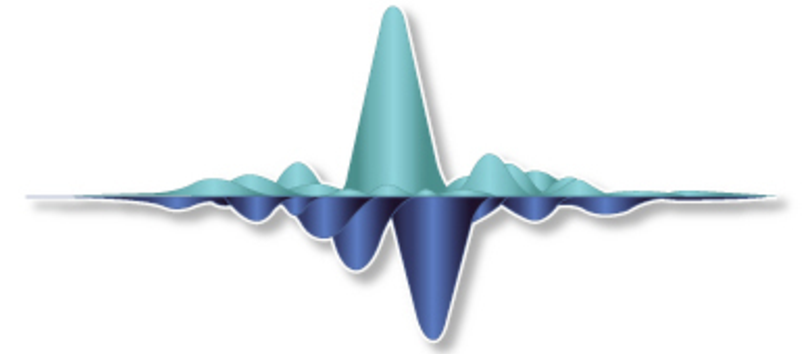
\includegraphics[height=1cm,width=2cm]{logo}
\end{textblock*}}

\maketitle

\begin{frame} \frametitle{Outline}
    \begin{itemize}
        \item Motivation
        \item Algorithm
        \item Synthetic Examples
        \item Real Examples
    \end{itemize}
\end{frame}

\begin{frame} \frametitle{Motivation}
    \begin{itemize}
        \item Processing tools that rely on sparsity or simplisity promotion can fail in the presence of static shifts.
	\item Many methods can solve for static shifts, but can we still process data with static shifts? 
	\item Here we adapt radon multiple attenuation and reconstruction to work in the presence of small static shifts.
    \end{itemize}
\end{frame}


%\begin{frame} \frametitle{Motivation}
%    \begin{itemize}
%        \item Here's a bullet.
%        \item And another bullet.
%        \item and one more.
%    \end{itemize}
%    \pause
%    \begin{itemize}
%        \item Another set of bullets.
%            \pause
%        \item But these are hidden from one another.
%            \pause
%        \item Which can be used to make animations.
%    \end{itemize}
%\end{frame}

%\begin{frame} \frametitle{POCS}
%    \Huge{$\nabla^2 u - \alpha \frac{\partial u}{\partial t} = %\delta(\mathbf{x},t)$}
%\end{frame}

\begin{frame} \frametitle{Projection Onto Convex Sets}
    \Large{$D^{k} = \alpha_1 D^{obs} + (1-\alpha_1 S)F_{D}^{-1}TF_{D}D^{k-1}$}

\bigskip

\bigskip
$\alpha_1 \rightarrow$ 1  when data are free of noise.
\end{frame}

\begin{frame} \frametitle{Projection Onto Convex Sets\\ {\color{red}with statics computation}}
    \Large{$D^{k} = \alpha_1 D^{obs}{\color{red}e^{-i\omega(1-\alpha_2)\tau^k}} + (1-\alpha_1 S)F_{D}^{-1}TF_{D}D^{k-1}$}

\bigskip

\bigskip
$\alpha_1 \rightarrow$ 1  when data are free of noise.
{\color{red}

$\alpha_2 \rightarrow$ 1  when data are free of statics.}
\end{frame}

\inputdir{syn5d}
% we could also use includegraphics here instead
%\begin{frame} \frametitle{Plots}
%    \plot{data1}{width=0.5\textwidth}{}
%\end{frame}

\begin{frame} \frametitle{Multiplots}
    \multiplot{2}{data1,data1_fk1k2}{width=0.45\textwidth}{}
\end{frame}

%\begin{frame} \frametitle{Multiplots}
%    \multiplot{2}{data1,data1}{width=0.45\textwidth}{}
%\end{frame}
%
%\begin{frame} \frametitle{example 2d all}
%    \plot{example_2d_all}{width=0.45\textwidth}{}
%\end{frame}
%
%\begin{frame} \frametitle{est data with without statics}
%    \multiplot{2}{estimated_data_without_statics,estimated_data_with_statics}{width=0.45\textwidth}{}
%\end{frame}

%\begin{frame} \frametitle{est data with without statics}
%    \multiplot{2}{high_resolution_radon_without_statics,high_resolution_radon_with_statics}{width=0.45\textwidth}{}
%\end{frame}

%\begin{frame} \frametitle{image d stat no stat}
%    \multiplot{5}{image_d_nostat,image_d_nostat_p,image_d_stat,image_d_stat_p,image_d_stat_pws}{width=0.45\textwidth}{}
%\end{frame}

%\begin{frame} \frametitle{original data}
%    \plot{no_missing}{width=0.45\textwidth}{}
%\end{frame}

%\begin{frame} \frametitle{no missing}
%    \plot{no_missing}{width=0.45\textwidth}{}
%\end{frame}

%\begin{frame} \frametitle{no missing pocs with statics}
%    \plot{no_missing_pws}{width=0.45\textwidth}{}
%\end{frame}

%\begin{frame} \frametitle{test2_all}
%    \plot{test2_all}{width=0.45\textwidth}{}
%\end{frame}


